% ------------------------------------------------------------------------------
% TYPO3 CMS 7.3 - What's New (English Version)
%
% @author	Michael Schams <schams.net>
% @license	Creative Commons BY-NC-SA 3.0
% @link		http://typo3.org/download/release-notes/whats-new/
% @language	English
% ------------------------------------------------------------------------------
% LTXE-CHAPTER-UID:		cc6b358d-f0ed36d3-f7a72fa2-af63ccfc
% LTXE-CHAPTER-NAME:	Backend User Interface
% ------------------------------------------------------------------------------

\section{Interfaz de Usuario de Backend}
\begin{frame}[fragile]
	\frametitle{Interfaz de Usuario de Backend}

	\begin{center}\huge{Capítulo 1:}\end{center}
	\begin{center}\huge{\color{typo3darkgrey}\textbf{Interfaz de Usuario de Backend}}\end{center}

\end{frame}

% ------------------------------------------------------------------------------
% LTXE-SLIDE-START
% LTXE-SLIDE-UID:		841d9eae-306bcdad-a7757d6f-d5bbeda5
% LTXE-SLIDE-ORIGIN:	111332b8-ac46a07a-319ed582-f873bc02 English
% LTXE-SLIDE-ORIGIN:	b4dc1576-57b4854f-26a32d85-11f7c52b German
% LTXE-SLIDE-TITLE:		Feature #66173: Allow page title edit by doubleclick
% LTXE-SLIDE-REFERENCE:	Feature-66173-AllowPageTitleEditByDoubleclick.rst
% ------------------------------------------------------------------------------
\begin{frame}[fragile]
	\frametitle{Interfaz de Usuario de Backend}
	\framesubtitle{Título de Página Title en Módulo Página y Lista}

	Los usuarios pueden editar los títulos de página en los módulos "Página" y "Lista" haciendo doble click en la cabecera del
	título o en el icono de edición.

	\begin{figure}
		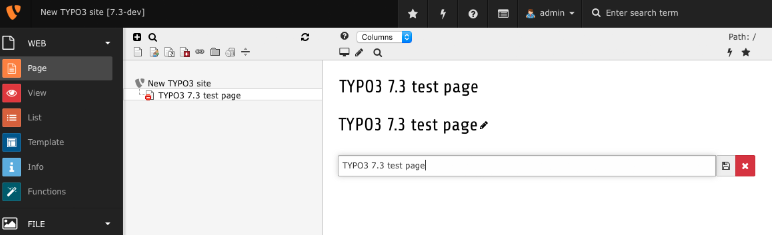
\includegraphics[width=0.9\linewidth]{BackendUserInterface/66173.png}
	\end{figure}

\end{frame}

% ------------------------------------------------------------------------------
% LTXE-SLIDE-START
% LTXE-SLIDE-UID:		3733e5c8-424c7d2d-0a36e0cb-6d9de63b
% LTXE-SLIDE-ORIGIN:	c17b263e-12512d4b-13d5389f-df1ec14e English
% LTXE-SLIDE-ORIGIN:	168b1424-1ebb2552-ed5bac3e-8a9ac737 German
% LTXE-SLIDE-TITLE:		Feature #67071: Processed files cleanup tool added in Install Tool
% LTXE-SLIDE-REFERENCE:	Feature-67071-ProcessedFilesCleanupToolAddedInInstallTool.rst
% ------------------------------------------------------------------------------
\begin{frame}[fragile]
	\frametitle{Interfaz de Usuario de Backend}
	\framesubtitle{Herramienta de Instalación: Borrar Ficheros Procesados}

	En su sección "Clean up", la Herramienta de Instalación proporciona una nueva función para eliminar
	ficheros procesados (p.e. previsualizaciones de imágenes) desde FAL ahora.\newline
	Esto es útil si se han cambiado los ajustes relacionados con los gráficos o tras una actualización de
	GraphicsMagick/ImageMagick para forzar que todas las imágenes sean regeneradas.

	\begin{figure}
		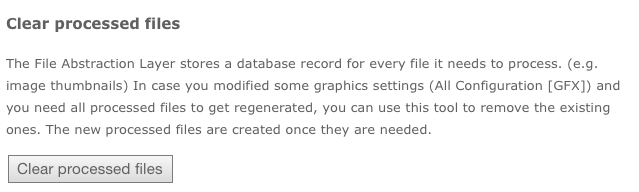
\includegraphics[width=0.6\linewidth]{BackendUserInterface/67071.png}
	\end{figure}

\end{frame}

% ------------------------------------------------------------------------------
% LTXE-SLIDE-START
% LTXE-SLIDE-UID:		393076f0-e321a73e-50003ded-ccb5ab0d
% LTXE-SLIDE-ORIGIN:	4662a0fc-e8a91f22-2f75e0bc-800e9b63 English
% LTXE-SLIDE-ORIGIN:	daa83c1e-08d2716b-de74cbda-42361551 German
% LTXE-SLIDE-TITLE:		Feature #67319: Add field "copyright" to EXT:filemetadata
% LTXE-SLIDE-REFERENCE:	Feature-67319-AddFieldCopyrightToEXTfilemetadata.rst
% ------------------------------------------------------------------------------
\begin{frame}[fragile]
	\frametitle{Interfaz de Usuario de Backend}
	\framesubtitle{Nuevo Campo en Metadatos FAL}

	Se ha añadido el campo "\textbf{Copyright}" a los metadatos de un registro FAL
	(extensión del sistema: \texttt{filemetadata}).

	\begin{figure}
		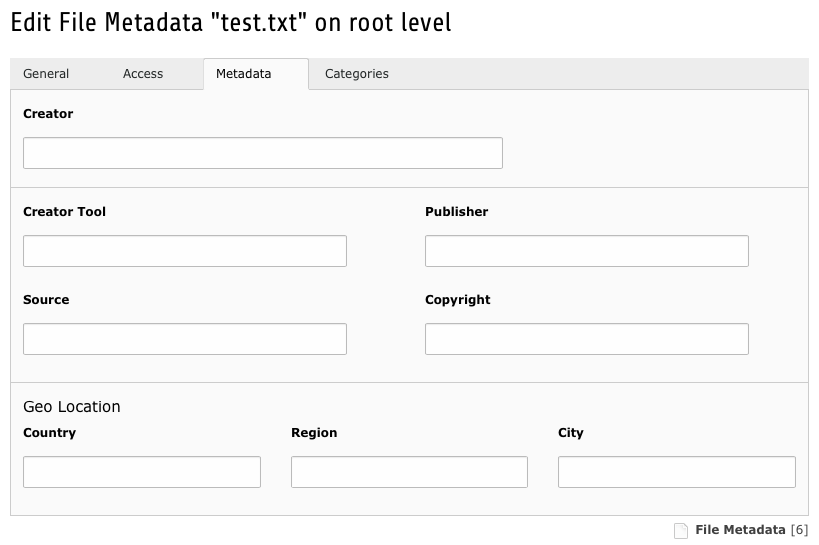
\includegraphics[width=0.6\linewidth]{BackendUserInterface/67319.png}
	\end{figure}

\end{frame}

% ------------------------------------------------------------------------------
